\section{Steps 2--3: executing a test case and the oracles}
\label{sec:oracles}

A fuzzer is only as good as its oracle. This section explains every way the
system decides that \pg did something wrong, and, just as important, every
rule that stops it from calling correct behaviour a bug.

\begin{figure}[h]
\centering
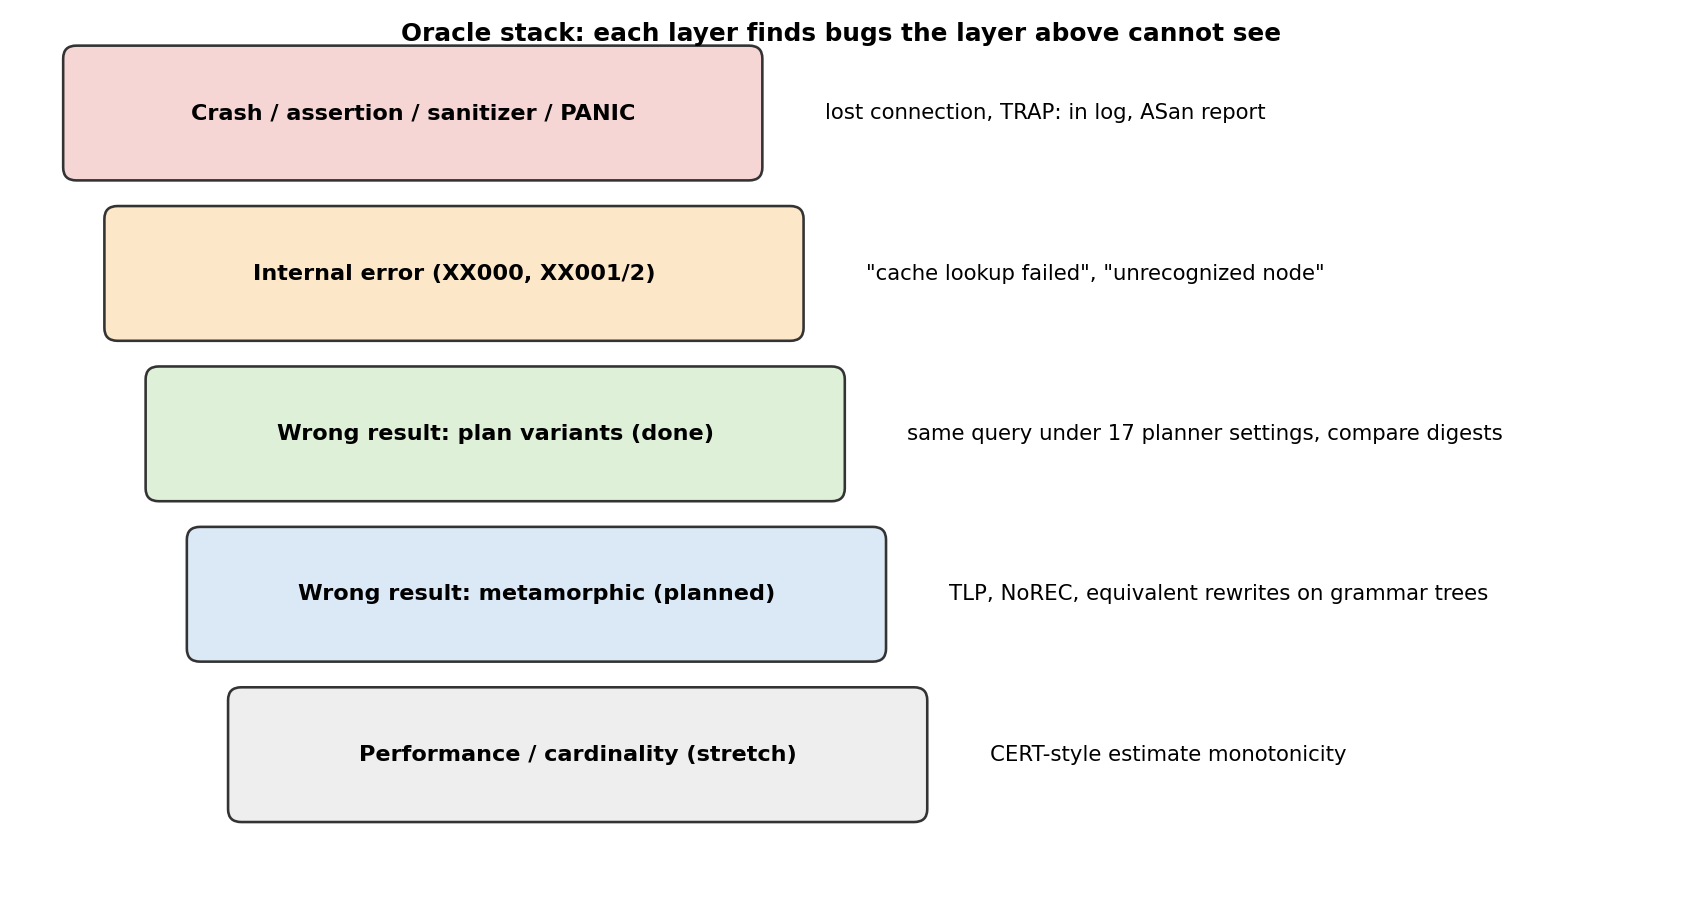
\includegraphics[width=0.85\linewidth]{oracle_stack.png}
\caption{The oracle stack: crash and error oracles see every statement;
plan-variant, metamorphic and cross-version oracles see deterministic queries.}
\end{figure}

\subsection{The executor}

\file{src/pgfuzz/reference/pg_executor.py} (741 lines) runs one test case on a
real server.
\begin{enumerate}
  \item \textbf{Isolation.} The test case runs inside one transaction; each
    statement in its own savepoint (\texttt{SAVEPOINT}, then \texttt{RELEASE} or
    \texttt{ROLLBACK TO}). At the end everything is rolled back, so the database
    is identical for the next test case. Statements that cannot run in a
    transaction (\texttt{VACUUM}, \texttt{CREATE INDEX CONCURRENTLY}) use
    \texttt{isolation: autocommit} plus a \texttt{reset\_sql} script.
  \item \textbf{Timeout} per statement (\texttt{statement\_timeout}, default 3 s
    in campaigns) so a slow plan cannot stall a worker.
  \item \textbf{Server log.} After each statement the executor reads new lines
    of the server log and looks for \texttt{TRAP:} (assertion),
    \texttt{PANIC:}, ``terminated by signal'', sanitizer reports and
    \texttt{BACKTRACE:} lines (\pg prints a C backtrace for internal errors
    when \texttt{backtrace\_on\_internal\_error = on}).
  \item \textbf{Crash recovery.} If the connection is lost, it waits for the
    postmaster to finish crash recovery (SQLSTATE 57P03 ``in recovery''),
    reconnects, and recreates the per-worker database if needed.
  \item \textbf{Digests.} For each successful query it computes an
    order-insensitive digest of the result (below) so it can compare results
    without storing them.
  \item \textbf{Oracle work} for each successful, deterministic query: plan
    variants, metamorphic checks, plan shape (\texttt{EXPLAIN (FORMAT JSON,
    COSTS OFF)} digest), optionally coverage sampling.
\end{enumerate}

\paragraph{Foreign-crash filter.} When one backend crashes, \pg restarts
\emph{all} backends; every other session sees ``terminating connection because
of crash of another server process'' (57P02). Each worker has its own server,
but our own manual PoC replay once crashed a server that a campaign was using
and the random arm was blamed. Now the executor records its backend PID
(\texttt{pg\_backend\_pid()}); crash evidence in the log must name that PID
(or a parallel worker of our own query), otherwise the event is classified
as \emph{foreign} and ignored (\texttt{\_foreign\_crash}).

\subsection{Classification}
\label{sec:classify}

\file{src/pgfuzz/eval/oracle.py} turns executor facts into one
\texttt{Outcome}, in priority order:
\begin{enumerate}
  \item log evidence: assertion, sanitizer, signal (crash), \texttt{PANIC};
  \item connection loss without an orderly SQLSTATE: crash;
  \item the SQLSTATE of a failing statement, by class:
    42601 $\rightarrow$ syntax; 42, 0A, 25, \dots{} $\rightarrow$ semantic;
    22, 23 \dots{} $\rightarrow$ runtime; 57014 $\rightarrow$ timeout;
    53, 54 $\rightarrow$ resource limit; \textbf{XX000 $\rightarrow$ internal
    error}; XX001/XX002 $\rightarrow$ data corruption. A short list of XX000
    messages that are really resource exhaustion (``out of memory'' in a
    hash table, etc.) is demoted;
  \item plan-variant facts: a variant that raised an internal error, or
    returned a different digest $\rightarrow$ \texttt{wrong\_result} (variant
    name recorded);
  \item metamorphic facts: a \emph{confirmed} mismatch $\rightarrow$
    \texttt{wrong\_result} with variant \texttt{mm:<kind>}; a CERT violation
    $\rightarrow$ \texttt{performance} (not a wrong answer).
\end{enumerate}
The outcomes are ordered by severity (ok $<$ syntax $<$ semantic $<$ runtime
$<$ timeout $<$ resource $<$ terminated $<$ performance $<$ wrong result $<$
internal error $<$ corruption $<$ panic $<$ assertion $<$ sanitizer $<$ crash).
The test case gets the most severe statement outcome; the index of that
statement is the \emph{culprit}. Bug candidates are: crash, assertion,
sanitizer, panic, corruption, internal error, wrong result, and (reported
separately) performance.

\subsection{Determinism: which queries may be compared at all}
\label{sec:eligible}

Comparing two runs of a query only makes sense if the correct answer is a
single multiset. \texttt{eligible(sql)} in \file{src/pgfuzz/eval/differential.py}
accepts a statement only if:
\begin{itemize}
  \item it is \texttt{SELECT}, \texttt{VALUES} or \texttt{TABLE} and contains no
    \texttt{INSERT/UPDATE/DELETE/MERGE/INTO} (no side effects);
  \item no \texttt{LIMIT}, \texttt{OFFSET}, \texttt{FETCH}, \texttt{TABLESAMPLE},
    \texttt{DISTINCT ON}, \texttt{FOR UPDATE/SHARE}, \texttt{SKIP LOCKED}
    (all choose \emph{some} rows, and which ones depends on the plan);
  \item no volatile function (\texttt{random}, \texttt{clock\_timestamp},
    \texttt{nextval}, \texttt{gen\_random\_uuid}, \texttt{pg\_sleep}, \dots, 42 names);
  \item no order-dependent window function (\texttt{row\_number}, \texttt{ntile},
    \texttt{lag/lead}, \texttt{first/last/nth\_value}) and no \texttt{ROWS}
    frame (ties are broken by the plan); \texttt{rank}, \texttt{dense\_rank},
    \texttt{percent\_rank}, \texttt{cume\_dist} are tie-safe and allowed;
  \item no order-sensitive aggregate without its own \texttt{ORDER BY}:
    \texttt{array\_agg}, \texttt{string\_agg}, \texttt{json(b)\_agg},
    \texttt{json(b)\_object\_agg}, \texttt{xmlagg}, \texttt{json\_arrayagg},
    \texttt{json\_objectagg}, \texttt{any\_value}, \dots;
  \item no \texttt{ARRAY(SELECT \dots)} without \texttt{ORDER BY} inside
    (added after candidate~1 of the bug hunt, a false positive).
\end{itemize}
The grammar helps: \texttt{@sorted\_agg} writes \texttt{array\_agg(x ORDER BY
x)}, so most aggregates the generator emits \emph{are} eligible.

\subsection{Result digests}
\label{sec:digest}

All values are fetched as text (\pg's own output format) and canonicalised:
\begin{itemize}
  \item \textbf{numeric scale:} \texttt{2.0}, \texttt{2.00} $\rightarrow$
    \texttt{2} (equal values; \texttt{DISTINCT}/\texttt{GROUP BY}/\texttt{UNION}
    may legitimately keep either representative -- found as a false positive in
    smoke run~1);
  \item \textbf{float $-0$:} $-0$ and $0$ compare equal, so either may survive;
  \item \textbf{float masking:} if the query has a floating-point aggregate or
    window (\texttt{sum}, \texttt{avg}, \texttt{stddev}, \texttt{corr},
    \texttt{regr\_*}, \texttt{percentile\_cont}, \texttt{OVER}), float columns
    are reduced to a class: \texttt{NaN}, \texttt{Infinity},
    \texttt{-Infinity} or ``finite''. Summation order changes the last digits
    legitimately; it cannot turn a finite value into NaN. (Masking
    \emph{everything} at first hid a re-injected bug: 0 vs NaN. That is why
    the class is kept.)
\end{itemize}
Rows are joined with separator bytes, sorted (multiset semantics), and hashed
with BLAKE2b (96 bits). Results above 10{,}000 rows are not compared.

\subsection{Oracle 1: plan variants (differential testing inside one server)}
\label{sec:variants}

The same query is re-run with \texttt{set\_config(name, value, true)} (local to
a savepoint, rolled back) under planner configurations. The settings change
\emph{how} \pg runs the query, never \emph{what} it returns, so any digest
difference is a bug (given eligibility). The 18 variants:

\begin{center}
\small
\begin{tabularx}{\linewidth}{lX}
\toprule
Variant & Settings (what it forces) \\
\midrule
\texttt{nestloop\_only} & hash and merge join off \\
\texttt{hashjoin\_only} & nested loop and merge join off \\
\texttt{mergejoin\_only} & nested loop and hash join off \\
\texttt{no\_hashagg} & sort-based grouping \\
\texttt{no\_sort\_opt} & no incremental sort, no presorted aggregate \\
\texttt{index\_scans} & seq scan and bitmap scan off \\
\texttt{seq\_scans} & index, index-only and bitmap scans off \\
\texttt{no\_memoize\_material} & no Memoize, no Material nodes \\
\texttt{parallel} & \texttt{debug\_parallel\_query=on}, zero parallel costs, 4 workers, leader not participating \\
\texttt{partitionwise} & partition-wise join and aggregate on \\
\texttt{no\_partition\_pruning} & partition pruning off \\
\texttt{geqo} & genetic optimizer from 2 relations \\
\texttt{no\_join\_reorder} & \texttt{join/from\_collapse\_limit = 1} (syntactic join order) \\
\texttt{tiny\_work\_mem} & \texttt{work\_mem=64kB}: hash joins batch, sorts spill to disk \\
\texttt{no\_reordering} & no GROUP BY / DISTINCT key reordering (PG 17/18 features) \\
\texttt{no\_self\_join\_elim} & self-join elimination off (new in PG 18) \\
\texttt{no\_eager\_agg} & eager aggregation off (new on master, Oct 2026) \\
\texttt{jit} & JIT compile everything (costs 0) \\
\bottomrule
\end{tabularx}
\end{center}

Settings unknown to the server are dropped at start (each variant is probed
once), so the same config works on 17, 18.6 and master. To keep throughput,
each query runs under \texttt{per\_query = 2} variants chosen
deterministically from a hash of the SQL text (\texttt{pick\_variants}): a
failure replays with the same variant, and over a campaign every variant is
used. A failure is \emph{materialised} for reports: the culprit statement is
preceded by explicit \texttt{SET} commands of the variant.

\paragraph{Why this finds bugs.} Each variant forces the planner down a
different code path (another join method, another aggregation strategy, a
parallel plan, spilling). Many optimizer bugs live in exactly one path.
Re-injected bug \texttt{rb-dfcf6fa7} was found this way in smoke run~2.

\subsection{Oracle 2: metamorphic rewrites of the derivation tree}
\label{sec:mm}

\file{src/pgfuzz/grammar/rewrite.py} (656 lines). For each eligible query, the
rewriter looks at its \emph{derivation tree} and the token span of each node,
and builds up to \texttt{per\_query} checks. A check has a left side (the
original query, or a variant of it) and a right side (the rewritten query);
both must return the same multiset. Kinds are sampled by weight (partition
checks apply to fewer queries, so they get larger weights: TLP-WHERE 6,
TLP-HAVING 5, TLP-agg 5, NoREC 3, expression 3, predicate 3, RLS 2, NOT NULL
1.5, CTE 1.5, fence 1.5, ORDER BY 1, CERT 1).

\begin{keybox}[Why do this on a tree and not on a string?]
SQLancer builds its own small queries so it knows their structure. We have
arbitrary, deeply nested queries from a 421-alternative grammar. The tree tells
us exactly which tokens are the \texttt{WHERE} predicate of \emph{this}
\texttt{SELECT} (not of a subquery), which expression has which type, which
level is grouped, which columns are in scope, and whether a node sits under an
outer join. A string rewrite would have to re-parse SQL and would get all of
these wrong some of the time; each mistake is a false positive.
\end{keybox}

\paragraph{Where a rewrite may apply.} Partition checks (TLP) apply to any
\texttt{select\_core} whose result is used as a multiset by the enclosing
query: the query itself, a subquery in \texttt{FROM}, a set-operation arm, an
\texttt{IN}/\texttt{EXISTS} subquery, a \texttt{LATERAL} subquery
(\texttt{MULTISET\_CONTEXTS}). Replacing a multiset by an equal multiset cannot
change the statement. A scalar subquery is \emph{not} such a context (it must
return one row), so it is not partitioned. Levels with window functions are
skipped (a window sees the whole partition; splitting the rows changes it).

\subsubsection*{The twelve kinds}

\begin{longtable}{p{0.17\linewidth}p{0.42\linewidth}p{0.33\linewidth}}
\toprule
\textbf{Kind} & \textbf{Rewrite (left $\equiv$ right)} & \textbf{Soundness conditions / targets} \\
\midrule
\endhead
\texttt{tlp\_where} & \texttt{SELECT .. FROM f} $\equiv$ \texttt{(.. WHERE p) UNION ALL (.. WHERE NOT p) UNION ALL (.. WHERE p IS NULL)} & Ternary logic partition (Rigger \& Su 2020). Not grouped. With \texttt{DISTINCT}: \texttt{UNION} instead, and only if all output types have a unique text form. Nested arms parenthesised so \texttt{INTERSECT} cannot regroup them. \\
\texttt{tlp\_having} & \texttt{.. GROUP BY k HAVING TRUE} $\equiv$ union of \texttt{HAVING p}, \texttt{NOT p}, \texttt{p IS NULL} & Grouped levels; group keys must have unique text form. Left side keeps \texttt{HAVING TRUE}: removing \texttt{HAVING} from a level without \texttt{GROUP BY} changes it from a one-group aggregate to a plain query (our false positive in smoke run~1). \\
\texttt{tlp\_agg} & \texttt{SELECT MIN(e) AS c0, COUNT(x) AS c1 FROM f} $\equiv$ \texttt{SELECT MIN(t.c0), SUM(t.c1) FROM (three partitions) t} & TLP for aggregates. Only combinable aggregates: MIN, MAX, SUM, COUNT$\rightarrow$SUM, BIT\_AND/OR/XOR, BOOL\_AND/OR, EVERY; no DISTINCT, FILTER or ORDER BY inside; every item exactly one call. \\
\texttt{norec} & \texttt{SELECT COUNT(*) FROM f WHERE p} $\equiv$ \texttt{SELECT COALESCE(SUM(CASE WHEN p THEN 1 ELSE 0 END),0) FROM f} & NoREC (Rigger \& Su 2020): the optimizer can use \texttt{p} in the first form (index, pushdown, join pruning) but must evaluate it per row in the second. \\
\texttt{expr} & replace one typed expression node $e$ by an equal one: \texttt{CASE WHEN TRUE THEN e END}, \texttt{COALESCE(e,e)}, \texttt{(SELECT e)}, \texttt{e+0}, \texttt{e*1}, \texttt{e||''}, \texttt{NOT NOT e}, \texttt{e AND TRUE}, \texttt{e OR FALSE}, \texttt{CASE WHEN e THEN TRUE WHEN NOT e THEN FALSE END} & EET-style (Jiang \& Su 2024). Rewrites are chosen \emph{by the node's type} (\texttt{+0} on float8 is excluded: $-0+0$ prints 0). No rewrite inside aggregates/windows for \texttt{(SELECT e)}. \textbf{\texttt{scalar\_sub} found BUG-02.} \\
\texttt{pred:in\_or} & \texttt{e IN (a,b)} $\equiv$ \texttt{(e=a) OR (e=b)} (also \texttt{NOT IN}) & Targets PG 18's OR-to-\texttt{= ANY} transformation. \\
\texttt{pred:cmp\_negate} & \texttt{a < b} $\equiv$ \texttt{NOT (a >= b)} & Exact under 3-valued logic for types with a B-tree total order. \\
\texttt{pred:between} & \texttt{x BETWEEN lo AND hi} $\equiv$ \texttt{x >= lo AND x <= hi} & Range/index-condition code. \\
\texttt{notnull} & \texttt{WHERE p} $\equiv$ \texttt{WHERE (p AND c IS NOT NULL)} for a NOT NULL column $c$ that $p$ already uses & Targets NOT-NULL-based simplification (PG 18). Not under outer joins (NULL-extended columns); not generated columns; $c$ must be in the scope of the predicate, not of a nested sub-select (\texttt{\_nested\_under}; a bug we fixed). \\
\texttt{order\_drop} & remove the statement's own \texttt{ORDER BY} & Multiset unchanged (no LIMIT, by eligibility). Exercises sort elimination and incremental sort. \\
\texttt{cte\_materialize} & \texttt{WITH x AS (..)} $\leftrightarrow$ \texttt{AS MATERIALIZED (..)} $\leftrightarrow$ \texttt{AS NOT MATERIALIZED} & Inlining vs materialisation of CTEs. \\
\texttt{table\_fence} & \texttt{t AS a} $\equiv$ \texttt{(SELECT * FROM t OFFSET 0) AS a} & \texttt{OFFSET 0} is an optimisation fence: no pull-up, no pushdown into the table. \\
\texttt{rls} & see below & information-flow oracle \\
\texttt{cert} & see below & performance oracle \\
\bottomrule
\end{longtable}

\paragraph{Example (TLP-WHERE), generated and rewritten by the tool:}
\begin{lstlisting}
-- original (left side keeps everything except WHERE)
SELECT t0_1.c0 AS c0 FROM t0 AS t0_1
-- right side
(SELECT t0_1.c0 AS c0 FROM t0 AS t0_1 WHERE ((t0_1.c0 > 5)))
UNION ALL
(SELECT t0_1.c0 AS c0 FROM t0 AS t0_1 WHERE NOT ((t0_1.c0 > 5)))
UNION ALL
(SELECT t0_1.c0 AS c0 FROM t0 AS t0_1 WHERE ((t0_1.c0 > 5)) IS NULL)
\end{lstlisting}

\paragraph{Confirmation.} A first mismatch is not enough: both sides are run
again. Only if both re-runs return the same digests as the first runs is the
mismatch \emph{confirmed}; otherwise it is \emph{unconfirmed} (the query is
not deterministic after all) and ignored. Errors on one side (``side errors'',
for example a rewrite that overflows) are counted, not reported, unless they are
internal errors.

\paragraph{LLM-proposed rewrites} come in as templates such as
\texttt{COALESCE(\{e\}, \{e\})} with a type; they are added to the same
\texttt{expr} pool after passing the rewrite gate (Section~\ref{sec:rwgate}).

\subsection{Oracle 3: the RLS leak oracle (information flow)}
\label{sec:rls}

\paragraph{Setup.} \file{src/corpus/rls.sql} creates role \texttt{pgfuzz\_rls}
(SELECT on all tables) and one policy on five tables:
\texttt{t0}: \texttt{(c0 \% 3) <> 0};
\texttt{t1}: \texttt{c1 IS NULL OR c1 < 30};
\texttt{t3}: \texttt{c1 IS NOT FALSE};
\texttt{tp}: \texttt{c0 > 10};
\texttt{ti}: \texttt{c1 IS DISTINCT FROM 'a'}.
The executor connects as a superuser, which bypasses RLS, so these policies
change nothing for the other oracles. As the role, 131 of the 203 rows of
\texttt{t0} are visible.

\paragraph{The check.} Left: the original query run with \texttt{SET LOCAL
ROLE pgfuzz\_rls} (policies apply). Right: the query run as superuser with
every protected table reference \texttt{t AS a} replaced by
\texttt{(SELECT * FROM t WHERE (policy)) AS a}. Both must be equal. A left side
with \emph{more} rows means a \textbf{leak}: the restricted role saw a row the
policy hides -- for example because a leaky function or an operator was pushed
below the security barrier, or a plan path forgot the policy qual. Fewer rows
means a wrong result.

\paragraph{Why it matters.} It connects the project to the course's
information-flow lectures (L21--22): the policy is a confidentiality label; the
oracle checks non-interference on concrete data. RLS bugs are security bugs
(\pg has had CVEs in this area, e.g. CVE-2023-2455 and CVE-2024-10976).
\emph{Measured:} 532 live checks on master, 0 false positives.

\subsection{Oracle 4: CERT (cardinality-estimation restriction testing)}
\label{sec:cert}

CERT (Ba \& Rigger, ICSE 2024): adding a restriction to a query must not
\emph{increase} the planner's row estimate. Left: \texttt{EXPLAIN} of the query
without its \texttt{WHERE}; right: \texttt{EXPLAIN} of the query. If the
estimate of the restricted query exceeds the unrestricted one, the outcome is
\texttt{performance} (a bad estimate leads to bad plans, but not to wrong
results). Restricted to ungrouped, non-\texttt{DISTINCT}, window-free levels,
where the monotonicity really holds. \emph{Measured:} 58 checks, 0 violations.
We report these separately and do not count them as wrong results.

\subsection{Oracle 5: cross-version (master vs 18.6)}
\label{sec:xversion}

\file{src/pgfuzz/reference/xversion_executor.py}. Every test case runs on the
server under test (master, assertions on) and on a reference (18.6 release).
For each statement that succeeded on both and is \texttt{xversion\_eligible},
the digests are compared; a difference is reported as a wrong result with
variant \texttt{xversion}, through the same path as plan variants.

\begin{itemize}
  \item \textbf{Why:} a new optimisation that is wrong under \emph{every}
    planner setting (no GUC turns it off) is invisible to plan variants but
    disagrees with a release that does not have it. Regressions in unreleased
    code are also what upstream fixes fastest (``open items'' before a
    release).
  \item \textbf{Exclusions:} clock and instance functions (\texttt{now},
    \texttt{current\_timestamp}, \texttt{version}, \texttt{pg\_backend\_pid},
    \texttt{current\_setting}, \dots) and functions whose behaviour changed
    \emph{on purpose}: \texttt{corr}, \texttt{regr\_r2/slope/intercept}
    (master commit \texttt{649828769} keeps $S_{xx}$ exactly 0 for constant
    input, so \texttt{corr(x,x)} over equal values is NULL on master, 1 on 18).
    We found that difference in smoke run~2 and confirmed it in the commit log.
  \item \textbf{Sequences} are not transactional: a \texttt{prelude\_sql}
    resets identity sequences on both servers before every test case.
  \item \textbf{Per-worker reference databases} \texttt{ref\_<worker>}, created
    by the executor (\texttt{create\_database}): four workers sharing one
    reference database raced on schema setup in smoke run~1.
  \item Statements that fail on only one side are counted
    (\texttt{test\_only\_ok}, \texttt{ref\_only\_ok}: new features, new errors)
    but not reported.
\end{itemize}
\emph{Measured:} 1{,}155 comparisons, 0 mismatches after the fixes.

\subsection{Signatures (deduplication)}
\label{sec:signatures}

Thousands of failing test cases may share one root cause. Each candidate gets
a signature (\file{src/pgfuzz/eval/signature.py}), strongest first:
\begin{description}
  \item[stack] top 5 symbolised frames of the backtrace, generic frames
    (\texttt{abort}, \texttt{ExceptionalCondition}, \texttt{PostgresMain},
    \dots) removed;
  \item[assert] assertion expression + source file;
  \item[message] SQLSTATE + error message with literals, numbers and hex
    abstracted (\texttt{N}, \texttt{?}, \texttt{H});
  \item[diff] for wrong results: oracle/variant + verb and SQL features of the
    culprit statement;
  \item[weak] crash without stack: signal + statement shape.
\end{description}
A failure directory is written only for the first test case of each new
signature. ``Unique bug candidates'' in the results are counted by signature,
and the strength is logged, because signature quality is a threat to validity.
